% Revision 4 -- new results subsections. Numbers in the text are from paper_rev4/generated/*.csv
% (make_assets.py); every table/figure is generated, none is typed by hand.
\subsection{Revision-4 results}\label{sec:results}

\begin{table*}[t]\centering\scriptsize
\caption{Simulation, UDP legitimate traffic: seconds with a target link above $\theta=0.8$ (mean $\pm$ 95\% CI over 30 seeds; lowest in bold).}\label{tab:sim_time}
\setlength{\tabcolsep}{3pt}
\begin{tabular}{llrrrrrrrr}
\toprule
Topology & Scen. & Static & ECMP & k-MP & Reactive & TE-LP & TE-$\Phi$ & RSDN & RSDN-v2\\
\midrule
Fat-tree & S3 & 60 & \textbf{0} & \textbf{0} & 28$\pm$3 & 2 & 2 & 6 & 6\\
 & S5 & 60 & \textbf{0} & \textbf{0} & 30 & 2 & 2 & 6 & 6\\
 & S6 & 600 & \textbf{0} & \textbf{0} & 300 & 2 & 2 & 6 & 6\\
 & S7 & 32 & \textbf{0} & \textbf{0} & 16 & 2 & 2 & 32 & 32\\
 & S8 & 14 & \textbf{0} & \textbf{0} & 8 & 2 & 2 & 6 & 6\\
 & S9 & 54 & \textbf{0} & \textbf{0} & 28 & 2 & 2 & 6 & 6\\
 & S10 & 33$\pm$6 & \textbf{0} & \textbf{0} & 17$\pm$3 & 2 & 2 & 8$\pm$1 & 8$\pm$1\\
 & S11 & 120 & \textbf{0} & \textbf{0} & 60 & 2 & 2 & 6 & 6\\
 & S12 & 120 & 20$\pm$17 & 48$\pm$22 & 62$\pm$4 & \textbf{6$\pm$8} & \textbf{6$\pm$8} & 12$\pm$8 & 8$\pm$1\\
 & S13 & 120 & 52$\pm$23 & 84$\pm$21 & 62$\pm$4 & \textbf{10$\pm$11} & 10$\pm$11 & 27$\pm$16 & 16$\pm$11\\
 & S14 & 120 & 70$\pm$20 & \textbf{0} & 62 & 15$\pm$4 & 16$\pm$3 & 50$\pm$0 & 50$\pm$0\\
\midrule
NSFNET & S3 & 60 & 60 & \textbf{0} & 15$\pm$5 & 2 & 2 & 6 & 6\\
 & S5 & 60 & 60 & \textbf{0} & 9$\pm$4 & 2 & 2 & 6 & 6\\
 & S6 & 600 & 600 & \textbf{0} & 151$\pm$57 & 22$\pm$41 & 2 & 65$\pm$68 & 26$\pm$40\\
 & S7 & 32 & 32 & \textbf{0} & 5$\pm$2 & 2 & 2 & 32 & 32\\
 & S8 & 14 & 14 & \textbf{0} & 3$\pm$1 & 2 & 2 & 6 & 6\\
 & S9 & 54 & 54 & 60$\pm$1 & 29$\pm$0 & 28$\pm$10 & 16$\pm$9 & 40$\pm$8 & \textbf{10$\pm$4}\\
 & S10 & 30$\pm$7 & 30$\pm$7 & 18$\pm$10 & 11$\pm$5 & 11$\pm$7 & \textbf{9$\pm$7} & 20$\pm$8 & 9$\pm$3\\
 & S11 & 120 & 120 & \textbf{0} & 31$\pm$11 & 2 & 2 & 17$\pm$13 & 6\\
 & S12 & 120 & 120 & 28$\pm$19 & 75$\pm$16 & \textbf{2} & \textbf{2} & 25$\pm$16 & 6\\
 & S13 & 120 & 120 & 120 & 115$\pm$6 & 92$\pm$19 & 85$\pm$20 & 109$\pm$13 & \textbf{51$\pm$21}\\
 & S14 & 120 & 120 & \textbf{4$\pm$7} & 57$\pm$6 & 36$\pm$14 & 20$\pm$3 & 65$\pm$7 & 50$\pm$1\\
\midrule
Internet2 & S3 & 60 & 60 & 16$\pm$10 & 28$\pm$3 & \textbf{2} & \textbf{2} & 11$\pm$6 & 6\\
 & S5 & 60 & 60 & \textbf{0} & 30 & 2 & 2 & 6 & 6\\
 & S6 & 600 & 600 & 320$\pm$114 & 300 & \textbf{2} & \textbf{2} & 204$\pm$106 & 6\\
 & S7 & 32 & 32 & \textbf{1$\pm$2} & 16 & 2 & 2 & 32 & 32\\
 & S8 & 14 & 14 & \textbf{1$\pm$1} & 8$\pm$0 & 2 & 2 & 6$\pm$1 & 6\\
 & S9 & 54 & 54 & 57$\pm$1 & 29$\pm$3 & 52$\pm$4 & 52$\pm$4 & 52$\pm$3 & \textbf{27$\pm$8}\\
 & S10 & 32$\pm$7 & 32$\pm$7 & 22$\pm$11 & 17$\pm$4 & 21$\pm$10 & 21$\pm$10 & 25$\pm$8 & \textbf{15$\pm$6}\\
 & S11 & 120 & 120 & 56$\pm$23 & 60 & \textbf{2} & \textbf{2} & 40$\pm$20 & 6\\
 & S12 & 120 & 120 & 72$\pm$22 & 62$\pm$4 & \textbf{2} & \textbf{2} & 40$\pm$20 & 6\\
 & S13 & 120 & 120 & 116$\pm$8 & 91$\pm$12 & 10$\pm$11 & 14$\pm$13 & 83$\pm$20 & \textbf{9$\pm$1}\\
 & S14 & 120 & 120 & 56$\pm$23 & 70$\pm$1 & \textbf{22$\pm$2} & 23$\pm$2 & 86$\pm$9 & 50$\pm$0\\
\midrule
G\'EANT & S3 & 60 & 60 & 34$\pm$11 & 26$\pm$4 & 33$\pm$11 & 25$\pm$11 & 15$\pm$8 & \textbf{6}\\
 & S5 & 60 & 60 & 16$\pm$10 & 17$\pm$5 & 23$\pm$11 & \textbf{2} & 6 & 6\\
 & S6 & 600 & 600 & 380$\pm$110 & 240$\pm$45 & 261$\pm$113 & \textbf{2} & 46$\pm$56 & 7$\pm$0\\
 & S7 & 32 & 32 & \textbf{2$\pm$3} & 6$\pm$2 & 17$\pm$6 & 13$\pm$5 & 32 & 32\\
 & S8 & 14 & 14 & \textbf{1$\pm$2} & 4$\pm$1 & 8$\pm$2 & 3$\pm$1 & 6 & 6\\
 & S9 & 54 & 54 & 59$\pm$1 & 28$\pm$2 & 25$\pm$10 & 14$\pm$8 & 11$\pm$5 & \textbf{7$\pm$2}\\
 & S10 & 33$\pm$6 & 33$\pm$6 & 19$\pm$10 & 13$\pm$4 & 18$\pm$8 & 10$\pm$5 & 12$\pm$5 & \textbf{9$\pm$2}\\
 & S11 & 120 & 120 & 68$\pm$23 & 50$\pm$8 & 49$\pm$22 & \textbf{2$\pm$0} & 7$\pm$0 & 7$\pm$0\\
 & S12 & 120 & 120 & 120 & 68$\pm$8 & 92$\pm$19 & 18$\pm$15 & 98$\pm$17 & \textbf{10$\pm$1}\\
 & S13 & 120 & 120 & 120 & 68$\pm$8 & 89$\pm$20 & 50$\pm$22 & 109$\pm$12 & \textbf{11$\pm$1}\\
 & S14 & 120 & 120 & 84$\pm$19 & 71$\pm$1 & 93$\pm$17 & \textbf{33$\pm$10} & 48$\pm$10 & 47$\pm$8\\
\bottomrule
\end{tabular}
\end{table*}

\paragraph{Overview (simulation, 30 seeds)}
Table~\ref{tab:sim_time} gives the seconds with a target above $\theta$ for every topology,
scenario and system; Tables~\ref{tab:paired_time} and~\ref{tab:paired_loss} summarise the paired
tests. Averaged over all attack scenarios and topologies, a target stayed above $\theta$ for
121\,s per run under static routing, 94\,s under static ECMP, 56\,s under simple reactive
rerouting, 45\,s under $k$-path multipath, 35\,s under ResilientSDN, 24\,s under TE-LP (min-max),
15\,s under ResilientSDN-v2 and 11\,s under TE-LP with the excess objective (TE-$\Phi$). Against
ResilientSDN, static routing is significantly worse in 33 of 48 cells and never better; simple
reactive is worse in 12 and better in 7: the pulse attack S7 on all four topologies (its one-poll
trigger reacts, ResilientSDN's three-poll trigger does not), G\'EANT S13, Internet2 S9 and NSFNET S8. Both LP baselines are significantly better in 28 (min-max)
and 35 (excess) cells and never worse; they use the same measurements but split flows fractionally
and react on the first poll.

\begin{table}[t]\centering\scriptsize
\caption{Paired comparison with ResilientSDN over all (topology, scenario) cells, seconds above $\theta$: number of cells in which the system is significantly lower / higher (Wilcoxon signed-rank on 30 seed-paired runs, Holm-corrected over all tests, $\alpha=0.05$) and median per-cell median difference.}\label{tab:paired_time}
\begin{tabular}{lrrrrr}
\toprule
System vs RSDN & cells & lower & higher & n.s. & median $\Delta$\\
\midrule
Static & 48 & 0 & 33 & 15 & +48.0\\
Static ECMP & 48 & 8 & 23 & 17 & +8.0\\
k-path multipath & 48 & 20 & 3 & 25 & -6.0\\
Simple reactive & 48 & 7 & 12 & 29 & +0.0\\
TE-LP (min-max) & 48 & 28 & 0 & 20 & -4.0\\
TE-LP (excess) & 48 & 35 & 0 & 13 & -4.0\\
ResilientSDN-v2 & 48 & 7 & 0 & 41 & +0.0\\
\bottomrule
\end{tabular}
\end{table}
\begin{table}[t]\centering\scriptsize
\caption{As Table~\ref{tab:paired_time}, for loss of the legitimate flows on the targets (\%).}\label{tab:paired_loss}
\begin{tabular}{lrrrrr}
\toprule
System vs RSDN & cells & lower & higher & n.s. & median $\Delta$\\
\midrule
Static & 48 & 0 & 20 & 28 & +0.0\\
Static ECMP & 48 & 2 & 15 & 31 & +0.0\\
k-path multipath & 48 & 12 & 4 & 32 & +0.0\\
Simple reactive & 48 & 0 & 16 & 32 & +0.0\\
TE-LP (min-max) & 48 & 15 & 1 & 32 & +0.0\\
TE-LP (excess) & 48 & 19 & 0 & 29 & +0.0\\
ResilientSDN-v2 & 48 & 1 & 0 & 47 & +0.0\\
\bottomrule
\end{tabular}
\end{table}
\begin{table*}[t]\centering\scriptsize
\caption{Simulation: loss of the legitimate flows that cross the target(s), \% (mean $\pm$ 95\% CI, 30 seeds).}\label{tab:sim_loss}
\setlength{\tabcolsep}{3pt}
\begin{tabular}{llrrrrrrrr}
\toprule
Topology & Scen. & Static & ECMP & k-MP & Reactive & TE-LP & TE-$\Phi$ & RSDN & RSDN-v2\\
\midrule
Fat-tree & S6 & 8.97$\pm$0.25 & \textbf{0.00} & \textbf{0.00} & 6.67$\pm$1.52 & 0.03$\pm$0.00 & 0.03$\pm$0.00 & 0.09$\pm$0.00 & 0.09$\pm$0.00\\
 & S9 & \textbf{0.00} & \textbf{0.00} & \textbf{0.00} & \textbf{0.00} & \textbf{0.00} & \textbf{0.00} & \textbf{0.00} & \textbf{0.00}\\
 & S11 & 9.09 & \textbf{0.00} & \textbf{0.00} & 7.01$\pm$1.44 & 0.15$\pm$0.00 & 0.15$\pm$0.00 & 0.45$\pm$0.00 & 0.45$\pm$0.00\\
 & S12 & 22.94$\pm$3.41 & 1.22$\pm$0.78 & \textbf{0.13$\pm$0.27} & 14.05$\pm$2.96 & 0.38$\pm$0.06 & 0.38$\pm$0.06 & 1.31$\pm$0.26 & 1.31$\pm$0.26\\
 & S13 & 26.93$\pm$2.91 & 1.30$\pm$0.92 & \textbf{0.34$\pm$0.41} & 19.01$\pm$3.13 & 0.45$\pm$0.05 & 0.45$\pm$0.05 & 1.70$\pm$0.38 & 1.53$\pm$0.18\\
 & S14 & 9.16$\pm$0.30 & 1.49$\pm$1.20 & \textbf{0.00} & 5.10$\pm$1.46 & 0.28$\pm$0.06 & 0.30$\pm$0.07 & 3.79$\pm$0.04 & 3.55$\pm$0.24\\
\midrule
NSFNET & S6 & 9.03$\pm$0.13 & 9.03$\pm$0.13 & \textbf{0.00} & 3.17$\pm$1.86 & 0.03$\pm$0.00 & 0.03$\pm$0.00 & 0.09$\pm$0.00 & 0.09$\pm$0.00\\
 & S9 & \textbf{0.00} & \textbf{0.00} & 10.02$\pm$1.79 & 43.50$\pm$4.18 & 0.29$\pm$0.13 & 0.33$\pm$0.15 & \textbf{0.00} & 0.02$\pm$0.04\\
 & S11 & 9.09 & 9.09 & \textbf{0.00} & 3.48$\pm$1.94 & 0.15$\pm$0.00 & 0.15$\pm$0.00 & 0.45$\pm$0.00 & 0.45$\pm$0.00\\
 & S12 & 9.09 & 9.09 & \textbf{0.00} & 8.96$\pm$2.58 & 0.15$\pm$0.00 & 0.15$\pm$0.00 & 0.45$\pm$0.00 & 0.45$\pm$0.00\\
 & S13 & 8.99$\pm$0.13 & 8.99$\pm$0.13 & 3.84$\pm$0.72 & 20.57$\pm$2.68 & \textbf{0.15$\pm$0.00} & \textbf{0.15$\pm$0.00} & 1.41$\pm$0.59 & 0.45$\pm$0.01\\
 & S14 & 9.09 & 9.09 & \textbf{0.00} & 6.24$\pm$1.78 & 0.20$\pm$0.03 & 0.26$\pm$0.05 & 2.47$\pm$0.68 & 3.67$\pm$0.21\\
\midrule
Internet2 & S6 & 9.09 & 9.09 & 0.17$\pm$0.36 & 10.82$\pm$0.82 & \textbf{0.03} & \textbf{0.03} & 0.09 & 0.09\\
 & S9 & \textbf{0.00} & \textbf{0.00} & 14.71$\pm$2.70 & 38.11$\pm$4.30 & 0.25$\pm$0.14 & 0.26$\pm$0.15 & \textbf{0.00} & \textbf{0.00}\\
 & S11 & 9.09 & 9.09 & \textbf{0.00} & 10.21$\pm$0.84 & 0.15$\pm$0.00 & 0.15$\pm$0.00 & 0.45$\pm$0.00 & 0.45$\pm$0.00\\
 & S12 & 9.16$\pm$0.15 & 9.16$\pm$0.15 & \textbf{0.07$\pm$0.14} & 8.81$\pm$1.63 & 0.15$\pm$0.00 & 0.15$\pm$0.00 & 0.60$\pm$0.29 & 0.46$\pm$0.01\\
 & S13 & 19.74$\pm$1.98 & 19.74$\pm$1.98 & 2.48$\pm$1.43 & 19.21$\pm$3.73 & \textbf{0.33$\pm$0.03} & \textbf{0.33$\pm$0.03} & 2.05$\pm$0.81 & 1.11$\pm$0.14\\
 & S14 & 9.09 & 9.09 & \textbf{0.00} & 9.68$\pm$1.00 & 0.22$\pm$0.07 & 0.40$\pm$0.16 & 3.51$\pm$1.00 & 3.79$\pm$0.04\\
\midrule
G\'EANT & S6 & 10.21$\pm$0.71 & 10.21$\pm$0.71 & 0.98$\pm$0.72 & 5.49$\pm$1.96 & 4.62$\pm$2.05 & \textbf{0.03$\pm$0.00} & 0.10$\pm$0.01 & 0.10$\pm$0.01\\
 & S9 & \textbf{0.00} & \textbf{0.00} & 32.96$\pm$4.56 & 46.33$\pm$4.21 & 0.11$\pm$0.10 & 0.13$\pm$0.11 & \textbf{0.00} & \textbf{0.00}\\
 & S11 & 10.44$\pm$0.79 & 10.44$\pm$0.79 & 0.57$\pm$0.59 & 6.00$\pm$2.46 & 4.69$\pm$2.18 & \textbf{0.17$\pm$0.01} & 0.52$\pm$0.04 & 0.52$\pm$0.04\\
 & S12 & 32.00$\pm$3.30 & 32.00$\pm$3.30 & 8.56$\pm$2.06 & 37.77$\pm$2.15 & 24.78$\pm$6.27 & \textbf{0.53$\pm$0.05} & 5.29$\pm$2.14 & 1.97$\pm$0.28\\
 & S13 & 26.27$\pm$2.05 & 26.27$\pm$2.05 & 7.12$\pm$1.42 & 28.06$\pm$2.21 & 18.19$\pm$5.31 & \textbf{0.54$\pm$0.21} & 4.72$\pm$1.47 & 1.61$\pm$0.16\\
 & S14 & 9.76$\pm$0.75 & 9.76$\pm$0.75 & 2.32$\pm$1.29 & 8.73$\pm$1.45 & 6.25$\pm$1.77 & \textbf{0.77$\pm$0.19} & 2.08$\pm$0.87 & 1.81$\pm$0.40\\
\bottomrule
\end{tabular}
\end{table*}
\begin{table*}[t]\centering\scriptsize
\caption{Simulation: flow moves per run (mean $\pm$ 95\% CI, 30 seeds). For TE-LP a move is any change of a flow's split by more than 1\%.}\label{tab:sim_reroutes}
\setlength{\tabcolsep}{3pt}
\begin{tabular}{llrrrrrrrr}
\toprule
Topology & Scen. & Static & ECMP & k-MP & Reactive & TE-LP & TE-$\Phi$ & RSDN & RSDN-v2\\
\midrule
Fat-tree & S3 & \textbf{0.0} & \textbf{0.0} & \textbf{0.0} & 99.7$\pm$5.6 & 1.0 & 1.0 & 1.0 & 1.0\\
 & S6 & \textbf{0.0} & \textbf{0.0} & \textbf{0.0} & 1610.5$\pm$96.3 & 2.9$\pm$0.1 & 2.9$\pm$0.1 & 1.0 & 1.0$\pm$0.1\\
 & S9 & \textbf{0.0} & \textbf{0.0} & \textbf{0.0} & 135.9$\pm$1.8 & 3.0 & 3.0 & 1.0 & 1.0\\
 & S11 & \textbf{0.0} & \textbf{0.0} & \textbf{0.0} & 312.4$\pm$15.4 & 2.9$\pm$0.1 & 2.9$\pm$0.1 & 1.0 & 1.0$\pm$0.1\\
 & S12 & \textbf{0.0} & \textbf{0.0} & \textbf{0.0} & 649.2$\pm$36.7 & 4.2$\pm$0.2 & 4.3$\pm$0.2 & 3.6$\pm$0.4 & 3.6$\pm$0.4\\
 & S13 & \textbf{0.0} & \textbf{0.0} & \textbf{0.0} & 1131.1$\pm$53.0 & 6.6$\pm$0.4 & 7.1$\pm$0.5 & 6.2$\pm$0.4 & 6.1$\pm$0.3\\
 & S14 & \textbf{0.0} & \textbf{0.0} & \textbf{0.0} & 373.8$\pm$25.1 & 19.6$\pm$4.9 & 21.3$\pm$4.3 & 12.3$\pm$0.3 & 12.1$\pm$0.1\\
\midrule
NSFNET & S3 & \textbf{0.0} & \textbf{0.0} & \textbf{0.0} & 60.5$\pm$20.5 & 1.1$\pm$0.1 & 1.0 & 1.0 & 1.0\\
 & S6 & \textbf{0.0} & \textbf{0.0} & \textbf{0.0} & 802.7$\pm$308.0 & 2.6$\pm$0.3 & 2.5$\pm$0.2 & 1.1$\pm$0.1 & 1.0\\
 & S9 & \textbf{0.0} & \textbf{0.0} & \textbf{0.0} & 356.4$\pm$23.3 & 6.6$\pm$1.5 & 8.6$\pm$1.3 & 1.6$\pm$0.4 & 3.6$\pm$0.6\\
 & S11 & \textbf{0.0} & \textbf{0.0} & \textbf{0.0} & 156.6$\pm$60.6 & 2.8$\pm$0.2 & 2.7$\pm$0.2 & 1.1$\pm$0.1 & 1.1$\pm$0.1\\
 & S12 & \textbf{0.0} & \textbf{0.0} & \textbf{0.0} & 386.6$\pm$77.9 & 5.5$\pm$0.4 & 4.9$\pm$0.3 & 2.1$\pm$0.1 & 2.0\\
 & S13 & \textbf{0.0} & \textbf{0.0} & \textbf{0.0} & 924.2$\pm$51.8 & 5.1$\pm$0.4 & 4.2$\pm$0.6 & 2.9$\pm$0.3 & 3.7$\pm$0.4\\
 & S14 & \textbf{0.0} & \textbf{0.0} & \textbf{0.0} & 244.2$\pm$35.1 & 19.6$\pm$4.6 & 25.4$\pm$3.3 & 11.7$\pm$1.1 & 11.9$\pm$0.3\\
\midrule
Internet2 & S3 & \textbf{0.0} & \textbf{0.0} & \textbf{0.0} & 117.2$\pm$14.8 & 1.6$\pm$0.3 & 1.0 & 0.9$\pm$0.1 & 1.1$\pm$0.1\\
 & S6 & \textbf{0.0} & \textbf{0.0} & \textbf{0.0} & 1689.9$\pm$77.5 & 2.3$\pm$0.2 & 2.2$\pm$0.2 & 1.1$\pm$0.1 & 1.0\\
 & S9 & \textbf{0.0} & \textbf{0.0} & \textbf{0.0} & 347.5$\pm$28.0 & 7.5$\pm$1.1 & 8.0$\pm$1.0 & 1.4$\pm$0.3 & 3.8$\pm$0.7\\
 & S11 & \textbf{0.0} & \textbf{0.0} & \textbf{0.0} & 323.3$\pm$18.3 & 2.2$\pm$0.2 & 2.1$\pm$0.2 & 1.2$\pm$0.2 & 1.1$\pm$0.1\\
 & S12 & \textbf{0.0} & \textbf{0.0} & \textbf{0.0} & 577.8$\pm$65.3 & 4.9$\pm$0.3 & 4.2$\pm$0.2 & 2.3$\pm$0.3 & 2.1$\pm$0.1\\
 & S13 & \textbf{0.0} & \textbf{0.0} & \textbf{0.0} & 864.1$\pm$107.1 & 7.4$\pm$0.5 & 7.0$\pm$0.9 & 4.8$\pm$0.4 & 5.4$\pm$0.6\\
 & S14 & \textbf{0.0} & \textbf{0.0} & \textbf{0.0} & 319.2$\pm$19.9 & 25.6$\pm$2.4 & 23.4$\pm$2.2 & 9.1$\pm$2.0 & 12.3$\pm$0.4\\
\midrule
G\'EANT & S3 & \textbf{0.0} & \textbf{0.0} & \textbf{0.0} & 98.2$\pm$17.2 & 0.7$\pm$0.4 & 1.2$\pm$0.2 & 1.0$\pm$0.2 & 1.0$\pm$0.1\\
 & S6 & \textbf{0.0} & \textbf{0.0} & \textbf{0.0} & 1326.3$\pm$273.0 & 2.0$\pm$0.8 & 1.9$\pm$0.3 & 1.3$\pm$0.2 & 1.3$\pm$0.2\\
 & S9 & \textbf{0.0} & \textbf{0.0} & \textbf{0.0} & 266.3$\pm$19.3 & 3.6$\pm$1.5 & 4.3$\pm$1.1 & 1.7$\pm$0.3 & 1.8$\pm$0.3\\
 & S11 & \textbf{0.0} & \textbf{0.0} & \textbf{0.0} & 280.7$\pm$49.6 & 1.9$\pm$0.7 & 2.2$\pm$0.3 & 1.3$\pm$0.2 & 1.3$\pm$0.2\\
 & S12 & \textbf{0.0} & \textbf{0.0} & \textbf{0.0} & 834.9$\pm$28.5 & 1.6$\pm$1.0 & 5.8$\pm$0.5 & 3.6$\pm$0.3 & 4.5$\pm$0.4\\
 & S13 & \textbf{0.0} & \textbf{0.0} & \textbf{0.0} & 1055.6$\pm$80.2 & 3.1$\pm$1.6 & 8.1$\pm$0.9 & 4.9$\pm$0.5 & 6.2$\pm$0.5\\
 & S14 & \textbf{0.0} & \textbf{0.0} & \textbf{0.0} & 354.2$\pm$27.3 & 1.9$\pm$1.0 & 15.2$\pm$3.1 & 8.0$\pm$1.5 & 10.5$\pm$1.7\\
\bottomrule
\end{tabular}
\end{table*}

\paragraph{Stability and cost}
ResilientSDN made 2.3 moves per run on average and 0.05 returns to an earlier path, against 388
moves and 379 returns for simple reactive rerouting (Table~\ref{tab:sim_reroutes}); TE-LP changed
4.5--5.4 flow splits per run and needs weighted select groups for every split flow
(rule changes per run: ResilientSDN 12.5, TE-LP 26--28, simple reactive 1\,967). Fig.~\ref{fig:tradeoff}
places each system by disruption and congestion time: ResilientSDN and v2 are the only single-path
systems close to the LP baselines.

\begin{figure}[t]\centering
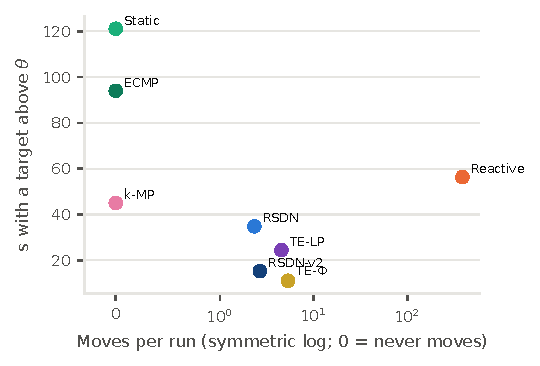
\includegraphics[width=\columnwidth]{figures/tradeoff}
\caption{Disruption (moves per run, log) against seconds a target is above $\theta$; means over all
attack scenarios, topologies and seeds (simulation).}\label{fig:tradeoff}
\end{figure}

\paragraph{WAN topologies, sustained and adversarial attacks (S6--S10)}
Fig.~\ref{fig:wan_adversarial} extends S6, S7, S8 and S10 to the three WANs. In the 600\,s
overload S6, ResilientSDN cut the time above $\theta$ from 600\,s (static) to 6\,s on the
fat-tree, 46\,s on G\'EANT, 65\,s on NSFNET and 204\,s on Internet2, and v2 to 6--26\,s on all
four; loss of the victim flows fell from about 9--10\,\% to 0.1\,\%. The Internet2 value
reproduces, in simulation, the hold that the emulation showed for Internet2 S11
(Sec.~\ref{sec:formulation}): with the sum drift, a 7--13-hop detour scores worse than the
congested one-hop link, so the deadband keeps the flow. The pulse attack S7 evades the trend
detector on every topology (ResilientSDN = static, 32\,s); the timed attack S8 is relieved within the
detection delay (6\,s). Under S10 (one of S7--S9 against randomised $N$ and cooldown) ResilientSDN
kept the target above $\theta$ for 8--25\,s against 30--33\,s for static routing; simple reactive was
lower on Internet2 and NSFNET, where S10 drew pulse runs, and v2 was at 8--15\,s.

\begin{figure*}[t]\centering
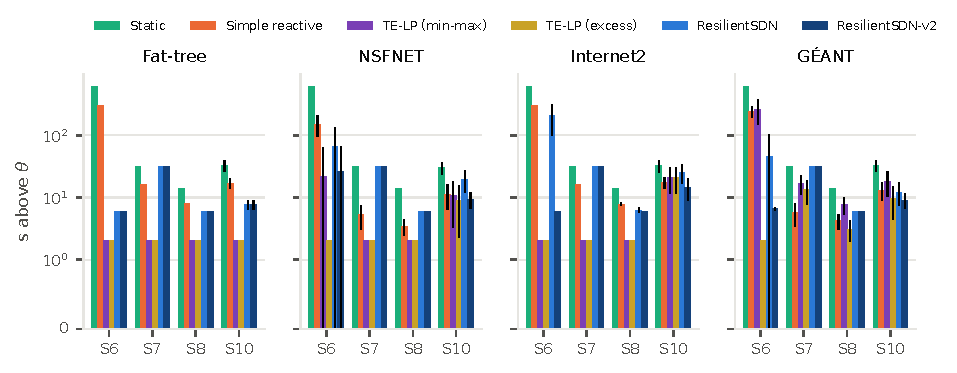
\includegraphics[width=\textwidth]{figures/wan_adversarial}
\caption{Seconds above $\theta$ for S6--S10 on all four topologies (simulation, mean and 95\,\% CI
over 30 seeds; symmetric-log axis).}\label{fig:wan_adversarial}
\end{figure*}

\paragraph{Closing the pulse loophole (v3)}
Table~\ref{tab:v3} adds the duty-cycle trigger (react when a link is above $\theta$ now and in at
least 3 of the last 6 polls) to ResilientSDN (+Duty) and to v2 (v3), over 13 scenarios, four
topologies and 30 seeds. It removes the pulse evasion of S7 on every topology (32 to 6\,s above
$\theta$) and lowers S10 from 16.2 to 13.6\,s (v2: 10.2 to 8.2\,s); averaged over all attacks, v3
keeps a target above $\theta$ for 11.8\,s, against 15.3\,s for v2 and 34.8\,s for ResilientSDN.
The cost is small: no move without an attack, neither in S1 nor under the legitimate bursts of SB
(where simple reactive rerouting made 14.8 moves per run and TE-$\Phi$ 2.4), unchanged secondary
congestion, and 0.1 more moves per run. In the paired tests (52 cells, Holm-corrected), v3 has
significantly less time above $\theta$ than ResilientSDN in 16 cells and more in none, and makes
significantly more moves in 8. The randomised sweep (Sec.~\ref{sec:sweep}) confirms the effect for
random pulse periods and duty cycles.
\IfFileExists{generated/tab_v3.tex}{\begin{table}[t]\centering\scriptsize
\caption{Duty-cycle trigger (simulation, 4 topologies $\times$ 30 seeds): +Duty adds it to the published ResilientSDN, v3 adds it to v2. False moves are reroutes when no attack is present.}
\label{tab:v3}
\begin{tabular}{lrrrr}
\toprule
 & RSDN & +Duty & RSDN-v2 & RSDN-v3\\
\midrule
False moves, S1 & 0.00 & 0.00 & 0.00 & 0.00\\
False moves, bursts (SB) & 0.00 & 0.00 & 0.00 & 0.00\\
s above $\theta$, S7 pulse & 32.0 & 6.0 & 32.0 & 6.0\\
s above $\theta$, S10 & 16.2 & 13.6 & 10.2 & 8.2\\
s above $\theta$, all attacks & 34.8 & 31.6 & 15.3 & 11.8\\
Victim loss \%, all attacks & 0.72 & 0.68 & 0.55 & 0.48\\
Secondary congestion & 0.05 & 0.05 & 0.35 & 0.36\\
Moves per run, all attacks & 2.3 & 2.4 & 2.7 & 2.8\\
\bottomrule
\end{tabular}
\end{table}}{}

\IfFileExists{generated/tab_wan_ext.tex}{\begin{table}[t]\centering\scriptsize
\caption{Mininet emulation of the scenarios added on the WANs in revision 4 (means over $n$ runs): legitimate loss (\%), seconds the target was above $\theta$, reroutes.}
\label{tab:wan_ext}
\setlength{\tabcolsep}{2.5pt}
\begin{tabular}{llrccc}
\toprule
Topology & Scen. & $n$ & Static & Reactive & RSDN\\
\midrule
NSFNET & S7 & 5 & 0.73 | 18 | 0.0 & 0.01 | 2 | 6.0 & 0.02 | 16 | 0.0\\
NSFNET & S8 & 5 & 0.64 | 12 | 0.0 & 0.00 | 6 | 12.6 & 0.06 | 6 | 1.2\\
NSFNET & S10 & 5 & 3.98 | 25 | 0.0 & 21.10 | 15 | 138.0 & 2.65 | 17 | 1.8\\
Internet2 & S7 & 5 & 0.00 | 27 | 0.0 & 0.43 | 12 | 46.4 & 0.00 | 27 | 0.0\\
Internet2 & S8 & 5 & 0.00 | 12 | 0.0 & 0.00 | 8 | 24.2 & 0.00 | 7 | 0.8\\
Internet2 & S10 & 5 & 0.92 | 34 | 0.0 & 19.30 | 20 | 213.2 & 1.31 | 32 | 2.2\\
G\'EANT & S7 & 3 & 0.00 | 26 | 0.0 & 0.00 | 2 | 5.3 & 0.00 | 26 | 0.0\\
\bottomrule
\end{tabular}
\end{table}}{}
\paragraph{WAN emulation of S6--S10}
% WAN-EMULATION-PARAGRAPH (filled in from generated/wan_ext_summary.csv when the campaign ends)

\paragraph{Multiple attacked links (S12, S13)}
With two or three simultaneously attacked links (Fig.~\ref{fig:multilink}), ResilientSDN's
single-link behaviour carries over on the fat-tree (12\,s for S12, 27\,s for S13) but not on the
WANs: 98 and 109\,s of 120\,s on G\'EANT, 40 and 83\,s on Internet2 (the long-detour hold again) and
25 and 109\,s on NSFNET. On NSFNET S13 no system kept the targets below $\theta$ for long (v2 51\,s,
TE-$\Phi$ 85\,s): three disjoint attacks on a 15-link network leave few detours with enough capacity. ResilientSDN-v2 reduced the time above $\theta$ to 6--16\,s on
fat-tree, Internet2 and G\'EANT and to 51\,s on NSFNET S13, and victim loss on G\'EANT from 5.3\,\%
to 2.0\,\% (S12). In S13, v2 is lower than TE-$\Phi$ (22\,s against 40\,s, mean over topologies),
whose six candidate paths per flow do not include the detours v2 finds within the hop limit.

\begin{figure*}[t]\centering
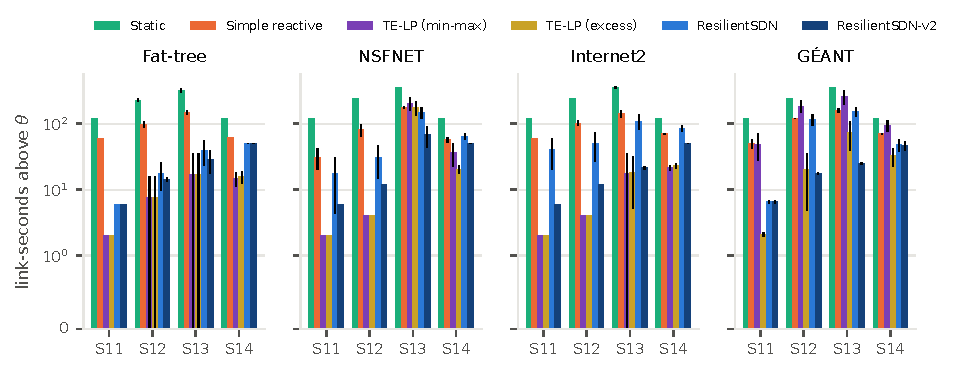
\includegraphics[width=\textwidth]{figures/multilink}
\caption{Link-seconds above $\theta$ summed over all targets: one target (S11), two (S12), three
(S13), and the adaptive attacker (S14). Simulation, 30 seeds.}\label{fig:multilink}
\end{figure*}

\paragraph{Adaptive rolling attacker (S14)}
When the attacker re-aims every 10\,s at the link the victims now share, every reactive defence
loses part of its advantage: ResilientSDN kept a target above $\theta$ for 48--86\,s of 120\,s
(static: 120\,s; v2: 47--50\,s), making 8--12 moves per run as it followed the attacker. TE-$\Phi$
did better on all four topologies (16--33\,s) and min-max TE-LP on three (it fails on G\'EANT,
94\,s, for the reason given above). $k$-path multipath was the most robust defence on fat-tree and
NSFNET (0--4\,s), since a fixed bot budget spread over three paths cannot push one link over
$\theta$, but not on Internet2 and G\'EANT (56--84\,s). Victim loss was 2--4\,\% for ResilientSDN,
9--10\,\% for static routing and below 1\,\% for TE-$\Phi$.

\paragraph{Presaturation (S9) and the cost of the fallback}
Simple reactive rerouting and $k$-path multipath both put traffic onto the pre-filled paths and lost
38--46\,\% and 10--33\,\% of the victim traffic on the WANs; the capacity filter kept ResilientSDN
at 0\,\%. The fallback of v2 halves the time above $\theta$ in S9 (27\,s to 12\,s), but by design
it may load a path above $\theta$: secondary congestion rises from 0.04 to 2.4 links per run on
average and to 6.7 on Internet2.
Table~\ref{tab:ablation_v2} separates the three v2 extensions: the bottleneck drift alone gives
most of the gain in S11--S14, the fallback acts only where no path passes the filter (S9, S13)
and is the one that causes the secondary congestion, and the severity order alone changes
nothing measurable. An operator who values ``no collateral congestion'' over relief time should
keep the fallback off; Proposition~\ref{prop:monotone} then holds.

\begin{table}[t]\centering\scriptsize
\caption{ResilientSDN-v2 ablation (simulation, mean over 4 topologies $\times$ 30 seeds): link-seconds above $\theta$ / victim loss (\%) / secondary congestion. Each extension alone, then all three (v2).}
\label{tab:ablation_v2}
\setlength{\tabcolsep}{2pt}
\begin{tabular}{lccccc}
\toprule
Scen. & RSDN & +Severity & +Fallback & +Bottleneck & RSDN-v2\\
\midrule
S9 & 27.2/0.00/0.04 & 27.2/0.00/0.03 & 12.4/0.00/2.22 & 24.8/0.00/0.03 & 12.5/0.00/2.36\\
S11 & 17.6/0.47/0.00 & 17.6/0.47/0.00 & 17.6/0.47/0.00 & 6.2/0.47/0.00 & 6.2/0.47/0.00\\
S12 & 53.8/1.92/0.02 & 51.9/2.03/0.02 & 55.6/1.56/0.07 & 15.8/1.06/0.03 & 13.9/1.05/0.08\\
S13 & 112.3/2.47/0.03 & 114.0/2.48/0.03 & 85.3/1.69/0.55 & 56.4/1.20/0.04 & 35.5/1.18/0.47\\
S14 & 62.2/2.96/0.43 & 62.2/2.96/0.43 & 62.0/2.99/0.48 & 50.7/3.15/0.10 & 49.2/3.21/0.12\\
\bottomrule
\end{tabular}
\end{table}

\paragraph{TCP goodput and flow-completion time}
With the legitimate flows as TCP transfers of 5\,MB (ideal FCT 2.0\,s), static routing raised the
mean FCT to 7.9--17\,s under overload (S6, S11--S13) and simple reactive rerouting to 4.5--16\,s,
partly because its oscillation moves the transfers between congested paths. ResilientSDN and v2
kept the mean FCT at 2.0--3.3\,s in every cell (Table~\ref{tab:sim_fct}, Fig.~\ref{fig:tcp_fct});
TE-$\Phi$ was closest to ideal (2.0--2.4\,s). The adaptive attacker (S14) is the scenario where
ResilientSDN's FCT rises most (2.6--3.3\,s), because victims are hit again after each move.
The fluid TCP model assumes that a TCP flow keeps at least 5\,\% of a saturated link. Re-running
S6 and S11--S14 with this floor at 0 and at 10\,\% (\floorCells{} topology--scenario cells, 30
seeds) changed the mean FCT of ResilientSDN, v2 and TE-$\Phi$ by at most 6\,\% and left the median
cell unchanged; static routing and simple reactive rerouting are more sensitive (up to
\floorMaxRel\,\%). The ranking changed in \floorFlips{} cells, but only between systems within
0.1\,s of each other (TE-$\Phi$, ResilientSDN, v2) or between static and simple reactive; the two
groups never swapped, so the TCP conclusions do not depend on the floor.

\begin{table*}[t]\centering\scriptsize
\caption{Simulation, TCP legitimate traffic: mean flow-completion time of 5\,MB transfers that start during the attack, s (mean $\pm$ 95\% CI, 30 seeds; ideal 2.0\,s).}\label{tab:sim_fct}
\setlength{\tabcolsep}{3pt}
\begin{tabular}{llrrrrrrrr}
\toprule
Topology & Scen. & Static & ECMP & k-MP & Reactive & TE-LP & TE-$\Phi$ & RSDN & RSDN-v2\\
\midrule
Fat-tree & S3 & 2.6$\pm$0.0 & 2.0$\pm$0.0 & \textbf{2.0} & 2.3$\pm$0.1 & \textbf{2.0} & \textbf{2.0} & 2.0 & 2.0\\
 & S6 & 7.9$\pm$0.0 & \textbf{2.0} & \textbf{2.0} & 6.5$\pm$0.9 & \textbf{2.0} & \textbf{2.0} & 2.0$\pm$0.0 & 2.0$\pm$0.0\\
 & S9 & 2.6$\pm$0.0 & \textbf{2.0} & \textbf{2.0} & 2.5$\pm$0.1 & 2.0$\pm$0.0 & 2.0$\pm$0.0 & 2.1$\pm$0.0 & 2.1$\pm$0.0\\
 & S11 & 7.9$\pm$0.0 & 2.0$\pm$0.1 & \textbf{2.0} & 6.6$\pm$0.9 & \textbf{2.0} & \textbf{2.0} & 2.0 & 2.0\\
 & S12 & 11.1$\pm$1.9 & 2.5$\pm$0.2 & 2.1$\pm$0.1 & 6.5$\pm$0.9 & 2.0$\pm$0.0 & \textbf{2.0$\pm$0.0} & 2.1$\pm$0.1 & 2.1$\pm$0.1\\
 & S13 & 12.5$\pm$2.1 & 2.4$\pm$0.2 & 2.2$\pm$0.1 & 7.1$\pm$1.1 & 2.0$\pm$0.0 & \textbf{2.0$\pm$0.0} & 2.2$\pm$0.1 & 2.1$\pm$0.1\\
 & S14 & 8.1$\pm$0.4 & 3.2$\pm$0.7 & \textbf{2.0} & 5.3$\pm$0.9 & 2.1$\pm$0.0 & 2.1$\pm$0.0 & 2.8$\pm$0.0 & 2.9$\pm$0.0\\
\midrule
NSFNET & S3 & 2.6$\pm$0.0 & 2.6$\pm$0.0 & \textbf{2.0} & 2.3$\pm$0.2 & \textbf{2.0} & 2.0$\pm$0.0 & 2.1$\pm$0.0 & 2.0\\
 & S6 & 7.9$\pm$0.0 & 7.9$\pm$0.0 & \textbf{2.0$\pm$0.1} & 4.9$\pm$1.8 & 2.1$\pm$0.1 & 2.0$\pm$0.1 & 2.0$\pm$0.1 & 2.0$\pm$0.1\\
 & S9 & 2.6$\pm$0.0 & 2.6$\pm$0.0 & 2.9$\pm$0.2 & 11.4$\pm$1.4 & 2.2$\pm$0.1 & 2.2$\pm$0.1 & 2.5$\pm$0.1 & \textbf{2.1$\pm$0.0}\\
 & S11 & 7.9$\pm$0.0 & 7.9$\pm$0.0 & \textbf{2.0} & 4.5$\pm$1.6 & \textbf{2.0} & \textbf{2.0} & 2.0$\pm$0.0 & 2.0$\pm$0.0\\
 & S12 & 7.9$\pm$0.0 & 7.9$\pm$0.0 & 2.0$\pm$0.0 & 4.6$\pm$0.8 & \textbf{2.0} & \textbf{2.0} & 2.1$\pm$0.0 & 2.0\\
 & S13 & 7.9$\pm$0.2 & 7.9$\pm$0.2 & 2.8$\pm$0.1 & 7.3$\pm$1.5 & 2.2$\pm$0.0 & 2.3$\pm$0.1 & 2.4$\pm$0.2 & \textbf{2.1$\pm$0.0}\\
 & S14 & 7.9$\pm$0.0 & 7.9$\pm$0.0 & \textbf{2.0$\pm$0.0} & 6.3$\pm$1.6 & 2.1$\pm$0.0 & 2.2$\pm$0.0 & 2.7$\pm$0.4 & 2.8$\pm$0.0\\
\midrule
Internet2 & S3 & 2.6$\pm$0.0 & 2.6$\pm$0.0 & 2.1$\pm$0.1 & 2.8$\pm$0.1 & \textbf{2.0} & \textbf{2.0} & 2.1$\pm$0.1 & 2.0\\
 & S6 & 7.9$\pm$0.0 & 7.9$\pm$0.0 & 2.2$\pm$0.2 & 10.8$\pm$1.5 & \textbf{2.0} & \textbf{2.0} & 2.2$\pm$0.1 & 2.0$\pm$0.0\\
 & S9 & 2.6$\pm$0.0 & 2.6$\pm$0.0 & 4.6$\pm$0.6 & 11.2$\pm$1.5 & 2.6$\pm$0.1 & 2.7$\pm$0.1 & 2.7$\pm$0.1 & \textbf{2.1$\pm$0.0}\\
 & S11 & 7.9$\pm$0.0 & 7.9$\pm$0.0 & 2.1$\pm$0.1 & 9.5$\pm$1.1 & \textbf{2.0} & \textbf{2.0} & 2.1$\pm$0.1 & 2.0$\pm$0.0\\
 & S12 & 8.0$\pm$0.2 & 8.0$\pm$0.2 & 2.1$\pm$0.1 & 6.1$\pm$1.1 & \textbf{2.0} & \textbf{2.0} & 2.1$\pm$0.1 & 2.0$\pm$0.0\\
 & S13 & 10.6$\pm$0.8 & 10.6$\pm$0.8 & 2.7$\pm$0.2 & 8.0$\pm$1.5 & \textbf{2.0$\pm$0.0} & 2.0$\pm$0.1 & 2.4$\pm$0.2 & 2.2$\pm$0.1\\
 & S14 & 7.9$\pm$0.0 & 7.9$\pm$0.0 & \textbf{2.1$\pm$0.1} & 9.3$\pm$1.3 & 2.2$\pm$0.2 & 2.1$\pm$0.0 & 3.3$\pm$0.5 & 2.9$\pm$0.1\\
\midrule
G\'EANT & S3 & 2.8$\pm$0.1 & 2.8$\pm$0.1 & 2.1$\pm$0.1 & 2.8$\pm$0.3 & 2.4$\pm$0.2 & 2.1$\pm$0.1 & 2.1$\pm$0.1 & \textbf{2.0$\pm$0.0}\\
 & S6 & 10.3$\pm$1.4 & 10.3$\pm$1.4 & 2.7$\pm$0.4 & 6.5$\pm$1.9 & 5.9$\pm$2.0 & 2.0$\pm$0.0 & 2.0$\pm$0.1 & \textbf{2.0$\pm$0.0}\\
 & S9 & 2.7$\pm$0.1 & 2.7$\pm$0.1 & 9.2$\pm$1.7 & 11.9$\pm$1.4 & 2.4$\pm$0.1 & 2.1$\pm$0.1 & 2.1$\pm$0.1 & \textbf{2.1$\pm$0.0}\\
 & S11 & 10.1$\pm$1.2 & 10.1$\pm$1.2 & 2.6$\pm$0.3 & 6.9$\pm$2.1 & 5.9$\pm$2.0 & \textbf{2.0$\pm$0.0} & 2.0$\pm$0.0 & 2.0$\pm$0.0\\
 & S12 & 17.0$\pm$2.2 & 17.0$\pm$2.2 & 4.3$\pm$0.5 & 16.3$\pm$2.5 & 13.4$\pm$3.2 & \textbf{2.0$\pm$0.1} & 2.8$\pm$0.4 & 2.2$\pm$0.1\\
 & S13 & 12.7$\pm$1.3 & 12.7$\pm$1.3 & 3.5$\pm$0.3 & 8.1$\pm$1.3 & 9.4$\pm$2.4 & \textbf{2.1$\pm$0.1} & 2.4$\pm$0.2 & 2.2$\pm$0.1\\
 & S14 & 9.4$\pm$1.1 & 9.4$\pm$1.1 & 3.7$\pm$0.9 & 8.7$\pm$1.5 & 6.7$\pm$1.5 & \textbf{2.4$\pm$0.3} & 2.6$\pm$0.8 & 2.4$\pm$0.3\\
\bottomrule
\end{tabular}
\end{table*}
\begin{figure*}[t]\centering
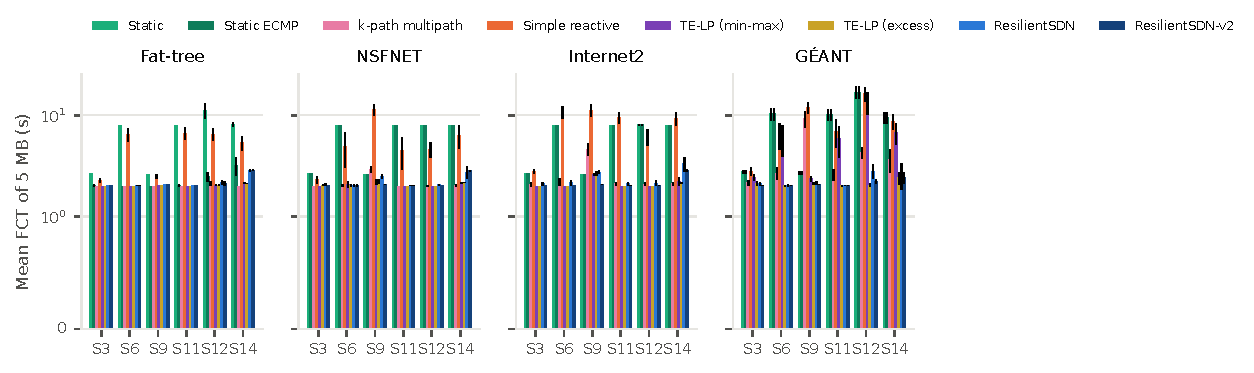
\includegraphics[width=\textwidth]{figures/tcp_fct}
\caption{Mean flow-completion time of the victims' 5\,MB TCP transfers (simulation, 30 seeds).}
\label{fig:tcp_fct}
\end{figure*}

\paragraph{ECMP against an ECMP-aware attacker}
With targets planned from static routes, ECMP and $k$-path multipath avoid the fat-tree attacks
altogether (Table~\ref{tab:sim_time}), which flatters them: the attack never reaches the link they
use. When the attacker picks host pairs that cross the target under both static and ECMP routing
(as Crossfire's route mapping would), ECMP is identical to static routing on every topology
(60 and 120\,s, Table~\ref{tab:sim_ecmp}), while ResilientSDN's results are similar to those with
the default attacker (the host pairs differ, so the values are not identical).

\begin{table*}[t]\centering\scriptsize
\caption{Simulation with an ECMP-aware attacker (attack pairs cross the target under both static and ECMP routing): seconds above $\theta$.}\label{tab:sim_ecmp}
\setlength{\tabcolsep}{3pt}
\begin{tabular}{llrrrrrrr}
\toprule
Topology & Scen. & Static & ECMP & k-MP & Reactive & TE-LP & RSDN & RSDN-v2\\
\midrule
Fat-tree & S3 & 60 & 60 & \textbf{0} & 26$\pm$4 & 2 & 6 & 6\\
 & S5 & 60 & 60 & \textbf{0} & 30 & 2 & 6 & 6\\
 & S9 & 54 & 54 & \textbf{0} & 27$\pm$2 & 2 & 6 & 6\\
 & S11 & 120 & 120 & \textbf{0} & 60 & 2 & 6 & 6\\
\midrule
NSFNET & S3 & 60 & 60 & \textbf{0} & 15$\pm$5 & 2 & 6 & 6\\
 & S5 & 60 & 60 & \textbf{0} & 9$\pm$4 & 2 & 6 & 6\\
 & S9 & 54 & 54 & 60$\pm$1 & 29$\pm$0 & 28$\pm$10 & 40$\pm$8 & \textbf{10$\pm$4}\\
 & S11 & 120 & 120 & \textbf{0} & 31$\pm$11 & 2 & 17$\pm$13 & 6\\
\midrule
Internet2 & S3 & 60 & 60 & 16$\pm$10 & 28$\pm$3 & \textbf{2} & 11$\pm$6 & 6\\
 & S5 & 60 & 60 & \textbf{0} & 30 & 2 & 6 & 6\\
 & S9 & 54 & 54 & 57$\pm$1 & 29$\pm$3 & 52$\pm$4 & 52$\pm$3 & \textbf{27$\pm$8}\\
 & S11 & 120 & 120 & 56$\pm$23 & 60 & \textbf{2} & 40$\pm$20 & 6\\
\midrule
G\'EANT & S3 & 60 & 60 & 34$\pm$11 & 26$\pm$4 & 16$\pm$9 & 8$\pm$4 & \textbf{6}\\
 & S5 & 60 & 60 & 10$\pm$8 & 13$\pm$5 & 25$\pm$11 & \textbf{6} & \textbf{6}\\
 & S9 & 54 & 54 & 59$\pm$1 & 29$\pm$0 & 26$\pm$10 & 11$\pm$5 & \textbf{7$\pm$2}\\
 & S11 & 120 & 120 & 72$\pm$22 & 46$\pm$9 & 49$\pm$22 & \textbf{6} & \textbf{6}\\
\bottomrule
\end{tabular}
\end{table*}
